%!TEX root = ../dissertation.tex
% this file is called up by thesis.tex
% content in this file will be fed into the main document

%: ----------------------- introduction file header -----------------------
% the code below specifies where the figures are stored
\graphicspath{{1-introduction/figures/}}

\chapter{Introduction}
\label{ch:introduction}

As listening is a core constituent of human perception, an essential component of artificial intelligence is \emph{machine listening}.
The purpose of machine listening research is to enable computers to process and understand sounds as humans do.
In recent years, there have been an unprecedented amount of successes in the field of \emph{machine learning}, a near-synonym to artificial intelligence with a connotation of statistical and/or probabilistic methodologies, which redefined what a computer vision or natural language processing systems can do and made previously unimaginable applications such as semi-autonomous driving\footnote{Fully autonomous driving is under active development; e.g. \href{https://tesla.com/autopilot}{Tesla Autopilot} and \href{https://waymo.com/}{Waymo}.} and a superhuman StarCraft-playing AI~\cite{vinyals2019alphastar} into reality.

In this context, this thesis focuses on improving the machine understanding of music in order to automatically transcribe music, which largely remains an unsolved problem despite decades of research.
The recent rapid development in \emph{deep learning} research, however, hints at many new possibilities for improving the performance or even achieving human-level accuracy in music transcription.

\section{Statement of Problem}\label{sec:statement}

\begin{figure}
	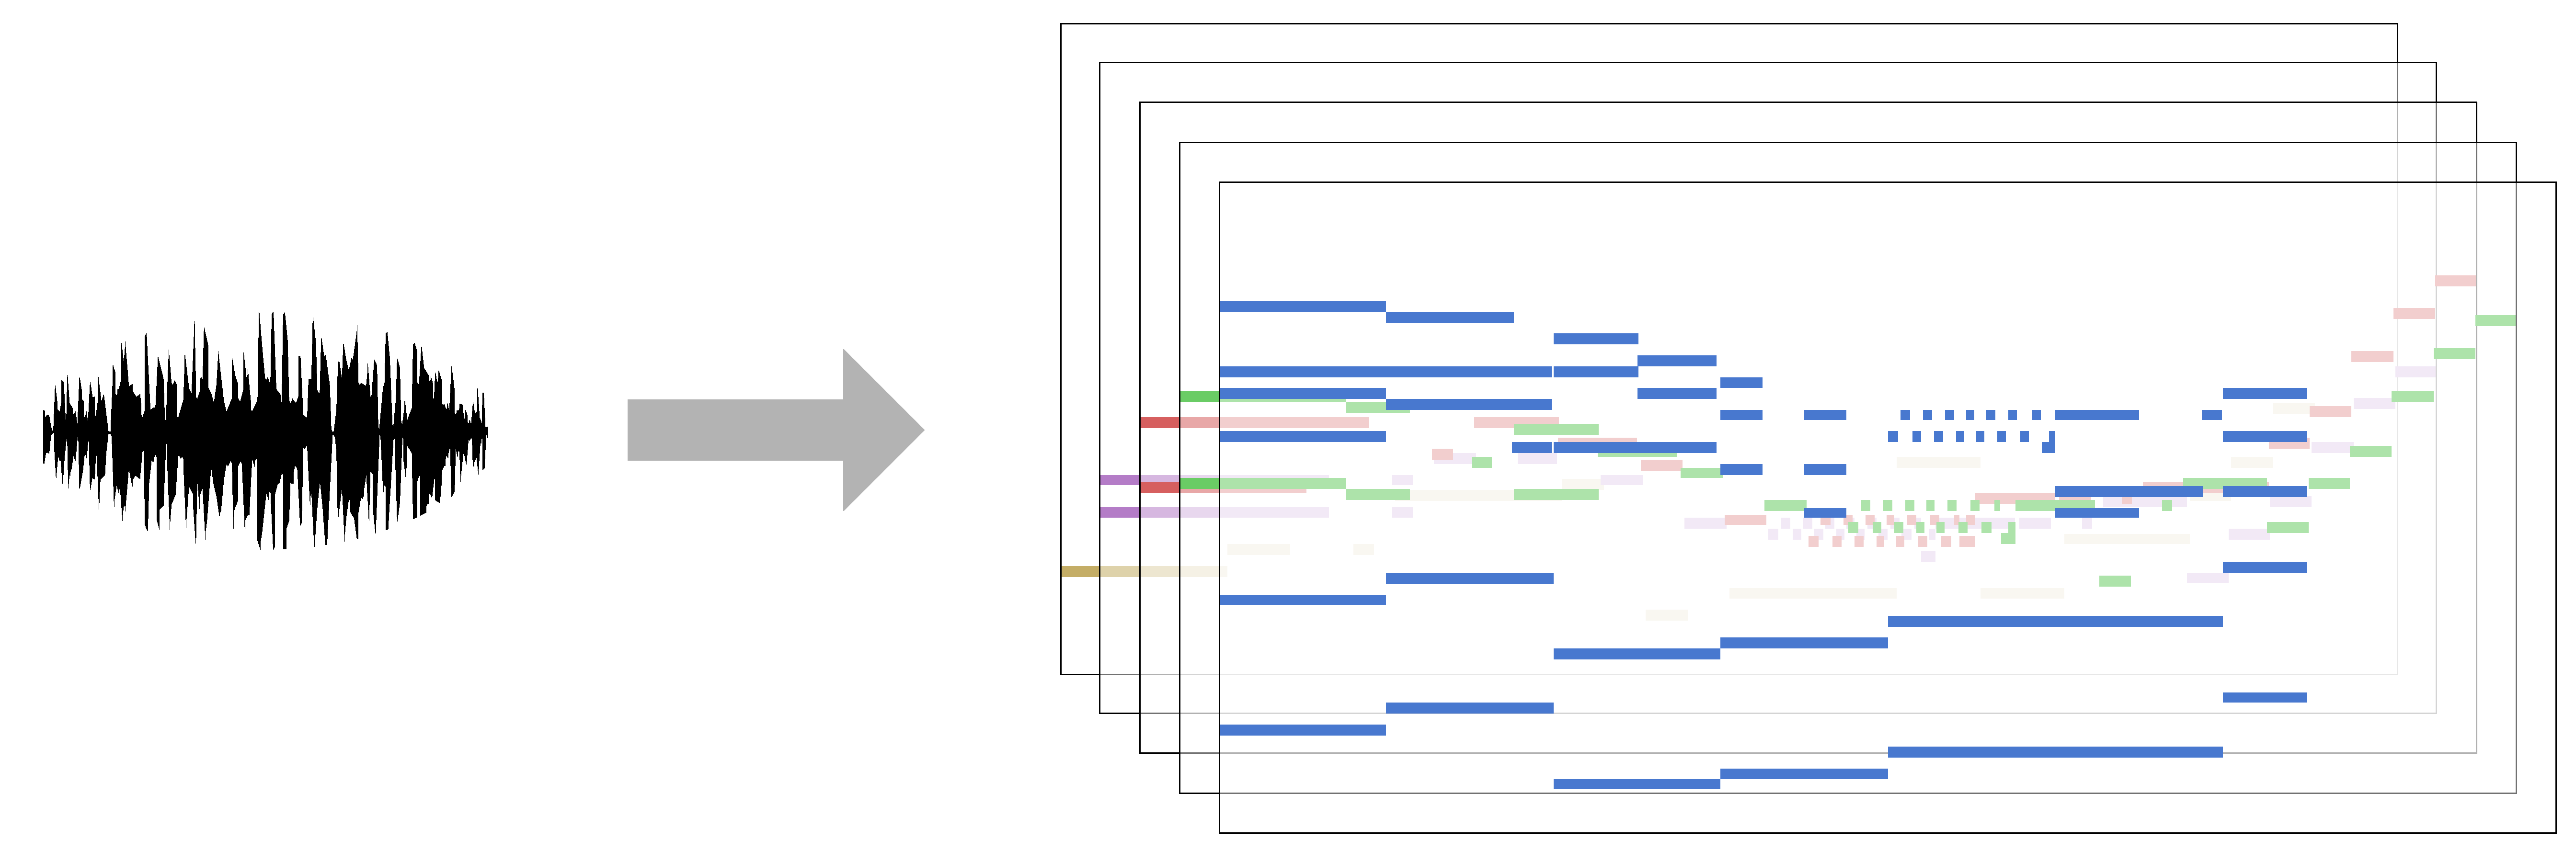
\includegraphics[width=\textwidth]{march-transcription.pdf}
	\caption{The automatic music transcription setup to be used in this thesis. Using per-instrument piano-roll representations is easier for machines to process, and avoids variability and subjectivity that may arise from symbolic and textual notations.} 
	\label{fig:transcription-to-piano-rolls}
\end{figure}

\emph{Automatic music transcription} (AMT) refers to an automated process that can identify musical events in the input audio and convert them into musical notations.
Historically, the definition of automatic music transcription varied by author, usually in terms of the form of the output representation.
In earlier works \cite{moorer1977transcription,piszczalski1977transcription}, the final output of the transcription system was to be the common music notation, i.e. a score, while later literature generalizes the problem by defining it as ``the analysis of an acoustic musical signal so as to write down the pitch, onset time, duration, and source of each sound that occurs in it" \cite{klapuri2006transcription} or ``the process of converting an acoustic musical signal into some form of musical notation" \cite{benetos2013amt}.
This thesis adopts per-instrument piano-rolls as the resulting representation of automatic music transcription, as shown in Figure \ref{fig:transcription-to-piano-rolls}, and defers the ``piano-roll to score" conversion as an out-of-scope task, which involves higher-level nontrivial tasks such as tempo and meter tracking, key signature detection, and music structure identification.
This can be justified since it allows the transcription model to focus on source separation and multi-pitch tracking, which are already highly challenging problems \cite{cemgil2006generative}.


To perform automatic music transcription, various properties of musical events, such as pitch, timbre, harmony, beats, etc., need to be defined and extracted from the audio.
In this sense, the setup of AMT is \emph{discriminative} in nature, meaning that it aims to identify different attributes from given audio, as opposed to \emph{generative} models concerning how to construct audio signals according to given conditions about those attributes.
Meanwhile, when a generative model is jointly trained with an encoder, it can learn to generate data samples from a small number of latent factors, while the encoder learns to extract those factors from the audio in a compact representation, as depicted in Figure \ref{fig:autoencoder}.
Recently, with the increased capacity of machine learning models and hardware, many \emph{deep generative models} have been proposed and shown to be capable of processing high-dimensional multimedia data.
Furthermore, significant research efforts have been made towards learning disentangled representations of data, meaning that the latent factors contain meaningful information that can be easily separated and isolated.
To this end, the goal of this thesis is to study representation learning methods powered by deep generative models, to obtain disentangled information from audio signals that can achieve better performance in music transcription.

\begin{figure}[t]
	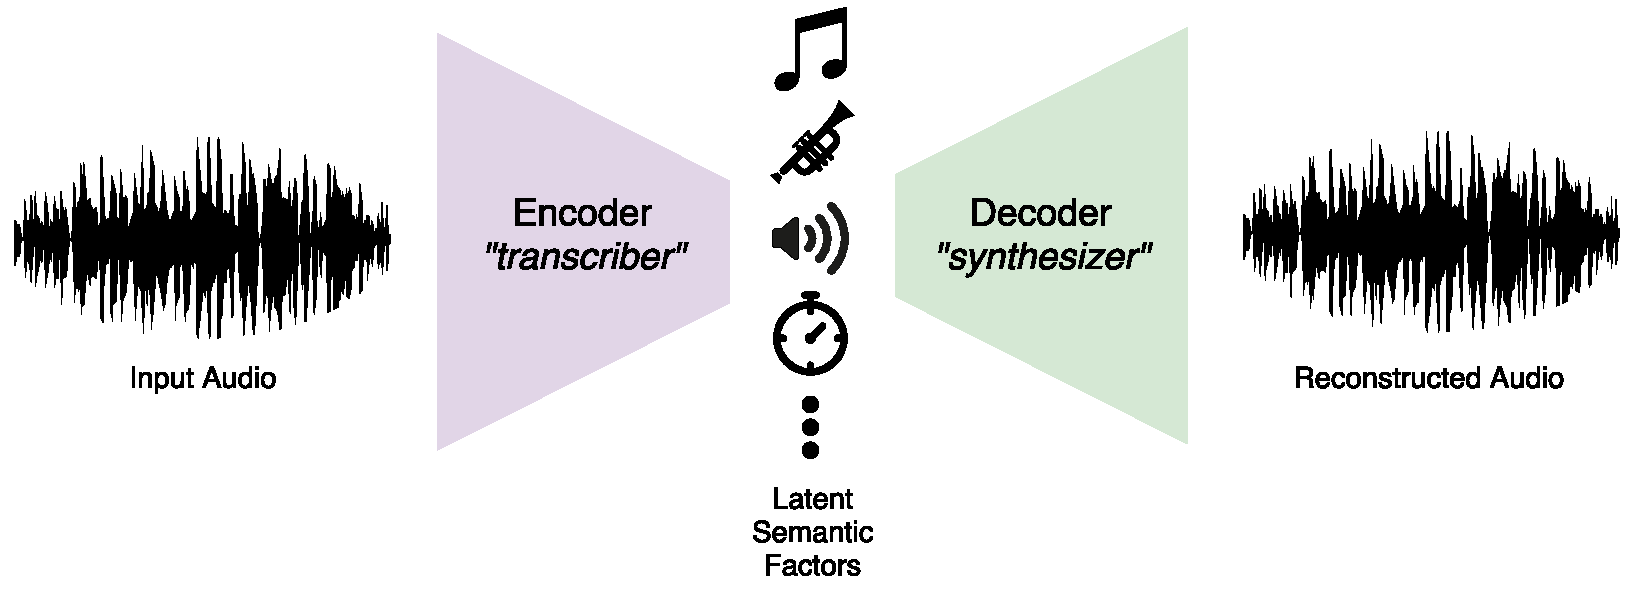
\includegraphics[width=\textwidth]{autoencoder.pdf}
	\caption{A generative model has to know all of necessary information required to reconstruct the audio data, including pitch, timbre, loudness, and duration. Generative models can be jointly trained with an encoder that finds those semantic information, giving a transcriber-synthesizer pair.}
	\label{fig:autoencoder}
\end{figure}

\section{Research Questions}\label{sec:subproblems}

To achieve the goal of improving music transcription with generative models, several research questions needs to be addressed. This thesis considers the following questions regarding the proposed approach towards automatic music transcription.

\vspace{1em}

\begin{enumerate}
\item What kinds of deep models and representations can be used for effectively extracting pitch from audio?
\item How does the choice of datasets affect the accuracy and the generalizability of a trained model?
\item How can we encode the concept of timbre in a way that is useful for music synthesis and transcription?
\item How can a transcription model make informed predictions incorporating the knowledge of a music language model?
\item Can a music synthesizer component based on a deep generative model be used to improve music transcription?
\end{enumerate}

\vspace{1em}

We aim to address each of these questions in the technical chapters of the thesis.
Through extensive experimental analysis in each chapter, we draw the conclusion on the effectiveness of deep generative models in the context of automatic music transcription.


\section{Limitations}\label{sec:limitations}

Because of the sophisticated and open-ended nature of automatic music transcription, it is necessary to define the scope of the tasks and data that this thesis will be concerned with.
The purpose of this section is to define those limitations in terms of the scope of music that the proposed AMT system can process, the required capability of symbolic music processing, and the need for perceptual studies regarding the validity of AMT systems.


\subsection{Scope of Music}

Music signals typically contain both harmonic and percussive sources. 
From a signal processing point of view, harmonic sounds are quasi-periodic and contain energy only at certain frequencies, roughly at the multiples of the fundamental frequency, whereas percussive or highly inharmonic sounds have aperiodic frequency spectra in which it is not possible to define a fundamental frequency.
Consequently, transcription models for harmonic sounds and percussive sounds require different techniques according to their nature.


This thesis will limit the focus on the transcription of harmonic sounds and therefore use the per-instrument piano roll notation (Figure \ref{fig:transcription-to-piano-rolls}) as the output representation.
This is a realistic trade-off to make, because of a number of reasons.
First, learning to simultaneously model harmonic and percussive sounds is a harder problem both conceptually and computationally.
Secondly, it is possible to plug a harmonic-only model into a pipeline consisting of harmonic-percussive source separation (HPSS) and a percussion transcription model as an alternative to a comprehensive approach.
Lastly, polyphonic transcription is considered to be the most difficult problem in the domain of automatic transcription, and it is sensible to tackle this as a standalone problem in the simplest possible setup.
Excluding percussive sounds will disallow using most of pop music tracks as-is, but multi-track datasets can still be utilized since they contain each track separately.


Additional limitations should be considered on the types of the instruments and their sound variations.
Depending on the instrument, the same score could be performed using a variety of expressive techniques, such as vibrato, tremolo, pizzicato, and the usage of mutes or harmonics, among others.
In order to accurately produce a piano roll transcription that is invariant to such techniques, the model has to be trained to classify them as nonessential information, requiring the availability of datasets with the annotations for those techniques.
While an ideal model should learn those concepts as humans do, too much timbral or temporal variation for an instrument will prevent the model from learning a consistent representation corresponding to the instrument.
Therefore, for the immediate purpose of this thesis, distributions of music signals that do not contain too much of said variations will be employed.


\subsection{Symbolic Processing of Notes}

As mentioned and justified in the problem statement (Section \ref{sec:statement}), by choosing per-instrument piano rolls as the output of transcription, concerns of symbolic music processing such as beat quantization and score typesetting are excluded from the scope of this study.
The difference between a piano roll output and a full human-readable score output becomes apparent when we compare the piano rolls in Figure \ref{fig:transcription-to-piano-rolls} with Figure \ref{fig:wedding-march-score}, which is the original score from which the piano rolls are plotted.
There are many aspects in producing the score output that are highly subjective and difficult to derive a consistent evaluation metric from, such as the interpretation of legatos or staccatos and the aesthetic choices for typesetting, providing an additional justification for using the piano roll notation.


\begin{figure}
	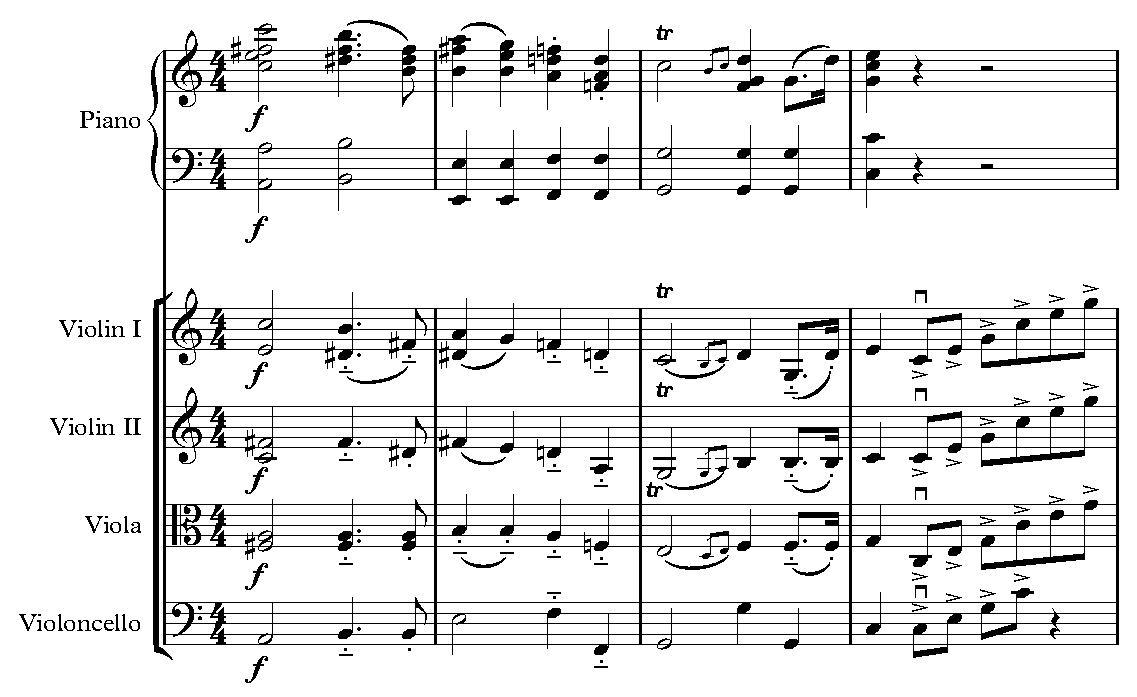
\includegraphics[width=\textwidth]{march-score.pdf}
	\caption{The full score notation of the music used to build the piano rolls in Figure \ref{fig:transcription-to-piano-rolls}. To fully recover this level of notations from the audio, the transcriber has to make many additional decisions than for the piano rolls, such as determining the key signature, time signature, clefs, dynamics, trills, bowing instructions, etc.}\label{fig:wedding-march-score}
\end{figure}


The MIDI file format is suitable for encoding data equivalent to per-instrument piano rolls, consisting of multiple tracks of \texttt{note\_on} and \texttt{note\_off} events with the corresponding timestamps.
MIDI will therefore be a supported output format of the proposed AMT system in addition to the piano roll representations, which can also be conveniently played back by media player software.
Music typesetting software such as Sibelius or Finale can render a MIDI file into score notation using the metadata in the file as well as some heuristics for beat quantization.
However, the readability of the score rendered from a transcribed MIDI file is limited, due to imperfect transcription and the absence of metadata such as the time and key signature.



\subsection{On the Need for Perceptual Studies}

This study of automatic music transcription is entirely quantitative and does not involve subjective tests on human participants.
We only aim to discover the systematic relations between audio signals and corresponding note sequences present in the datasets we use for training.
However, music is essentially a perceived notion, and thus are the core qualities of sound --- pitch, timbre, and loudness --- which are the output of automatic transcription.
For this reason, manually annotating polyphonic music is an error-prone process, where any two annotators may produce drastically different annotations.
Although this problem of inaccuracy and subjective difference is often overcome by using a ground-truth dataset synthesized from known frequency information, the gap still persists between what a model can learn from synthesized audio and how it will respond to real-world sounds.
This thesis uses both kinds of datasets, from synthesized and recorded audio signals, and thus the real-world applicability of each of the proposed models should be carefully examined.

The goal of automatic transcription is at a lower level than for tasks such as  chord recognition and melody tracking, which may incur even more subjective disagreements caused by the imprecise definitions of chords and melodies.
Being directly related to the physical concept of fundamental frequency, pitch is relatively precisely defined in this sense, and formulating automatic music transcription as an audio-to-piano-roll conversion mostly eliminates the ambiguity that exists in chord recognition and melody tracking.
There exist some cases where the mathematical definition of fundamental frequency still cannot be applied for all pitched sounds, such as the Shepard tone \cite{shepard1964circularity} where the pitch of a harmonic sound fails to be consistently mapped to a fundamental frequency.
However, disregarding these few edge cases, this study assumes that the piano roll notation can convey an objective transcription for many practical purposes, allowing us to postulate AMT as a mathematical problem which does not require experiments on human subjects.

\section{Need for Study}

The nature of music transcription is multifold; to create a complete transcription, one has to identify all instruments, onsets, dynamics, and the pitch traces for every instrument present in the music, and it would still be far from achieving the human-level accuracy.
The need for this study arises naturally, not only because this is an intriguing problem in the intersection of music and technology that has remained unsolved for decades, but also because the solution to this problem can provide practical benefits to many applications.

In order to bolster the need for this study, a few of such applications are introduced in this section, followed by discussions on the advantages of employing generative models as a means of better capturing musical semantics.
A brief perspective on AMT is presented in the context of wider AI research, followed by the organization of the chapters.


\subsection{Applications of Automatic Music Transcription}\label{sec:applications}

Many applications of the techniques in the realm of automatic music transcription is on interactive music systems.
\citeA{vercoe1984performer} proposed a quest for a \emph{synthetic performer}, which can listen, perform, and learn in the context of live performance.
Relevant sub-fields include automatic \emph{real-time accompaniment} \cite{dannenberg1985accompaniment} based on dynamic programming was one of the first successful demonstrations of AMT techniques, and \emph{Score following}, a general term referring to the synchronization of a computer with a performer playing a known score \cite{orio2003following}.
An offline music-to-score matching algorithm can also be applied to intelligent audio editors \cite{dannenberg2003following}.

\emph{Music recommender systems} can combine many kinds of information for improved music retrieval and personalization \cite{celma2010music}.
Content-based music recommender systems can utilize not only the metadata but also the audio content, and methods using timbral \cite{magno2008recommendation}, temporal \cite{li2007recommender}, and tonal features \cite{lu2009recommendation} have been introduced.
These music recommender systems can be further improved when the complete information on each domain is made available through AMT.

AMT system can help create databases for query-by-humming \cite{ghias1995humming} by automatically estimating melody annotations, where users can retrieve music by humming an excerpt of the song.
Such databases can also facilitate large-scale musicological analyses \cite{abdallah2015british}, as well as the development of computer-aided music composition \cite{agostini2013aid} that incorporates musicological knowledge.


\subsection{Generative Modeling for Fully Capturing Semantics}

Being ``generative'' means that a model is capable of generating new samples in the domain of the original data.
Generation in the symbolic domain creates new musical scores, and a generative model in the audio domain creates audio waveforms.
These two kinds of generative systems are familiar to computer music artists and are referred to as algorithmic composition \cite{fernandez2013ai} and sound synthesis \cite{cook2002synthesis} models.
This thesis defines the term ``generative model'' more specifically, as a model that can learn the distribution of provided data and can sample new samples in the original distribution.
This differs from the term ``generative'' used in computer music in a sense that it aims to accurately model the probability distribution and learn to regenerate the real-world audio to be used in music transcription, rather than focusing on the artistic aspects of generating new kinds of sounds and music.

By learning to generate data using fewer parameters than the scale of the dataset, a model has to discover the underlying natural features from the distribution of data.
In music transcription, these features correspond to the musical concepts such as pitch, timbre, and rhythm.
Philosophically, this idea follows what Richard Feynman once wrote on his blackboard, \emph{``What I cannot create, I do not understand''} and \emph{``Know how to solve every problem that has been solved''}.
He meant that the marker for truly understanding something is the ability to construct it completely from scratch.
Studies on generative models have an advantage of not requiring explicitly labeled data, and they hence tend to take self-supervised or unsupervised learning approaches.
\citeA{lecun2016unsupervised} introduced unsupervised learning as a cake, with supervised learning as icing and reinforcement learning as the cherry on the top, by which he meant that generative models need to predict at a much larger scale of information and should be able to learn the ``common sense''.

\begin{figure}
	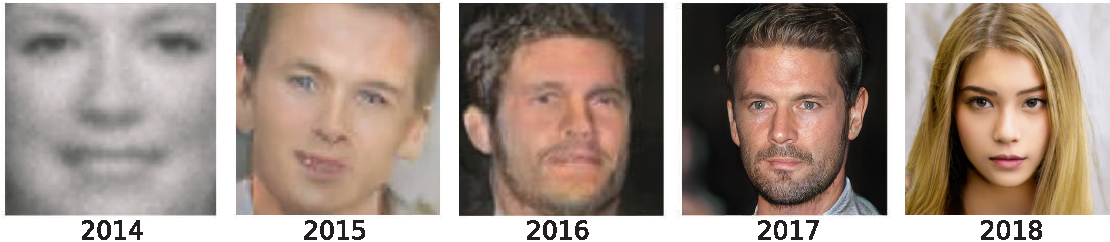
\includegraphics[width=\textwidth]{generative-evolution.pdf}
	\caption{Increasingly realistic qualities of the generated faces using generative adversarial networks as shown in \protect\cite{brundage2018malicious}; images are taken from \protect\cite{goodfellow2014gan}, \protect\cite{radford2015dcgan}, \protect\cite{liu2016cogan}, \protect\cite{karras2017pggan}, and \protect\cite{karras2019stylegan}.} 
	\label{fig:generative-evolution}
\end{figure}


Inherently, unsupervised learning is less well-defined than supervised learning, and this is the reason why unsupervised learning is sometimes synonymous with clustering, because finding clusters is usually as much an unsupervised learning system can do.
However, the recent success of deep learning introduced a new breed of generative models, enabling the end-to-end generation of complex data such as photos and audio signals.
\emph{Generative adversarial networks} (GAN) \cite{goodfellow2014gan} are the most notable among them, and their performance in generating realistic images has been improving at an extraordinary pace, as shown in Figure \ref{fig:generative-evolution}.
Combined with the various techniques for manipulating the semantic information in GANs as will be introduced in Section \ref{ch:deeplearning}.\ref{sec:gan}, this hints at completely new kinds of generative methodologies for audio processing.


In this context, this thesis aims to design and develop improved methods for automatic music transcription powered by deep generative models.
The idea specifically hypothesizes that by training a generative model, it is possible to learn disentangled representations, from which the information necessary for transcription can be easily extracted, as depicted in Figure \ref{fig:autoencoder}.
By doing so, the ultimate objective is to build an end-to-end model that connects the piano roll representation to audio signals, in order to perform automatic music transcription --- obtaining the most likely piano roll representation for given a audio waveform.


\subsection{On the Broader Context of Machine Listening in AI Research}

Using generated audio data and generative models is partly motivated by the fact that synthesized music is more prevalent and perceptually more familiar to people than synthesized texts or pictures.
Many commercial music tracks are often produced entirely using software instruments, except for the vocal parts.
This suggests that synthesized and generated audio may more accurately model the distribution of the real audio data to be transcribed.
This generative approach also aligns well with how actual musicians transcribe music, where they match given audio with their knowledge of how the instruments sound when played in a certain combination of rhythms and melodies.
Therefore it is reasonable to claim that machines should also be able to perform in a similar way, provided that a proper representation of knowledge about the music and instruments is available.

The task of automatic music transcription shares many common values with other machine learning tasks, such as image segmentation, machine translation, and speech recognition, in the sense that the core task is to build an intelligent system that can extract and process useful information conveyed in complex signals.
This is an essence of artificial intelligence (AI)
--- a system that perceives its environment and takes actions that maximizes the utility \cite{russell2009ai} --- 
where an intelligent system has to understand the semantics of complex data coming from the environment in order to perform well in its tasks.
To this end, the problem of automatic music transcription is not just an intriguing task in music technology but will also be a key component of the AI-enabled future society, constituting a musical component of the artificial general intelligence (AGI), in the form of advanced machine musicianship \cite{rowe2003musicianship}.


\subsection{Organization of The Thesis}


This thesis examines the possibility of using deep generative models to learn relevant musical concepts and inform a music transcription model to incorporate them.
There exists a rich history of research aiming at the understanding of musical sounds and automatic music transcription; to validate this claim as a feasible research direction and place this thesis in the context of this continuum of research, Chapter \ref{ch:mir} provides a review of the standard methods and the current state of the art in automatic music transcription research.
Deep learning techniques are employed as a building block throughout this thesis, and a general introduction to deep learning and deep generative models is provided in Chapter \ref{ch:deeplearning}, with a focus on generative adversarial networks.

In Chapter \ref{ch:monophonic}, we first consider a subproblem of music transcription, i.e. monophonic pitch estimation, and learn that convolutional neural networks predicting two-dimensional time-frequency representations can constitute an effective strategy, which we build and extend in the subsequent chapters.
Chapter \ref{ch:synthesis} examines the applications of deep generative models in music analysis and synthesis tasks, by introducing a WaveNet-based music synthesis model that learns a multi-dimensional timbre representation.
In Chapter \ref{ch:adversarial}, generative adversarial networks are used to apply a music language model that can help improve a piano transcription model.
In Chapter \ref{ch:timbre}, we combine the analysis and synthesis methods developed in the preceding chapters and present a multi-instrument polyphonic music transcription system.
Finally, concluding remarks are provided in Chapter \ref{ch:conclusions}.


